\documentclass{article}
\usepackage[utf8]{inputenc}
\usepackage[spanish]{babel}
\usepackage{graphicx}
\usepackage{anysize}
\usepackage{fancyhdr} 
\usepackage[export]{adjustbox}
\usepackage{titlesec}
\usepackage{enumitem}
% \usepackage{hyperref}
% \usepackage{float}
% \usepackage{tabu}

% Izquierda, derecha, arriba, abajo
\marginsize{2cm}{2cm}{1.2cm}{1.5cm} 
\renewcommand{\familydefault}{\sfdefault}
\decimalpoint%

\graphicspath{{assets/}{feedback.assets/}}

\setlength{\parindent}{0in}
\titleformat*{\section}{\large\bfseries}

\newcommand{\materia}{CCNA V7}
% \newcommand{\clave}{}
% \newcommand{\profesor}{Ing. Rodriguez Campos \textsc{Jorge Alberto}}
\newcommand{\grupo}{1}
\newcommand{\semestre}{2021-1}

\newcommand{\alumno}{Francisco Pablo \textsc{Rodrigo}}

\newcommand{\actividad}{Módulo 01}
\newcommand{\titulo}{Feedback}

\newcommand{\fechaEntrega}{27 de octubre de 2020}

%%%%%%%%%%%%%%%%%%%% ENCABEZADO %%%%%%%%%%%%%%%%%%%%%%%%%%%%
\pagestyle{fancy}
\fancyhf{}
\renewcommand{\headrulewidth}{0pt}
% \setlength{\headsep}{0.3in}

\begin{document}
%%%%%%%%%%%%%%%%%%% DATOS MINI PORTADA %%%%%%%%%%%%%%%%%%%%%%%%
\begin{minipage}[t]{0.7\linewidth}
    \vspace{-1cm}
    % \large{\textbf{UNAM}} \large{\textbf{FI}} \\
    \large{\textbf{\materia}}\\
    \large{\textbf{Grupo \grupo}}\\
    % \large{\textbf{Profesor:} \profesor}\\ [1.5cm]
    \textbf{\actividad}\\
    \textbf{\titulo} \\

    \large{\textbf{Alumno:} \alumno} \\
    \textbf{Fecha:} \fechaEntrega%
\end{minipage}\hfill
\begin{minipage}[t]{0.2\linewidth}
    \vspace{-1.2cm}
    \begin{flushright}
        % 
\includegraphics[width=2cm]{fiblack}
        
\includegraphics[width=2cm]{unam.jpg}\\
        % \vspace{10cm}
        \large{\semestre}    
    \end{flushright}
\end{minipage}
\vspace{5mm}
%%%%%%%%%%%%%%%%%%% CONTENIDO %%%%%%%%%%%%%%%%%%%%%%%%

\textbf{Segmento de red asignado}: \texttt{192.168.7.0/24}\\
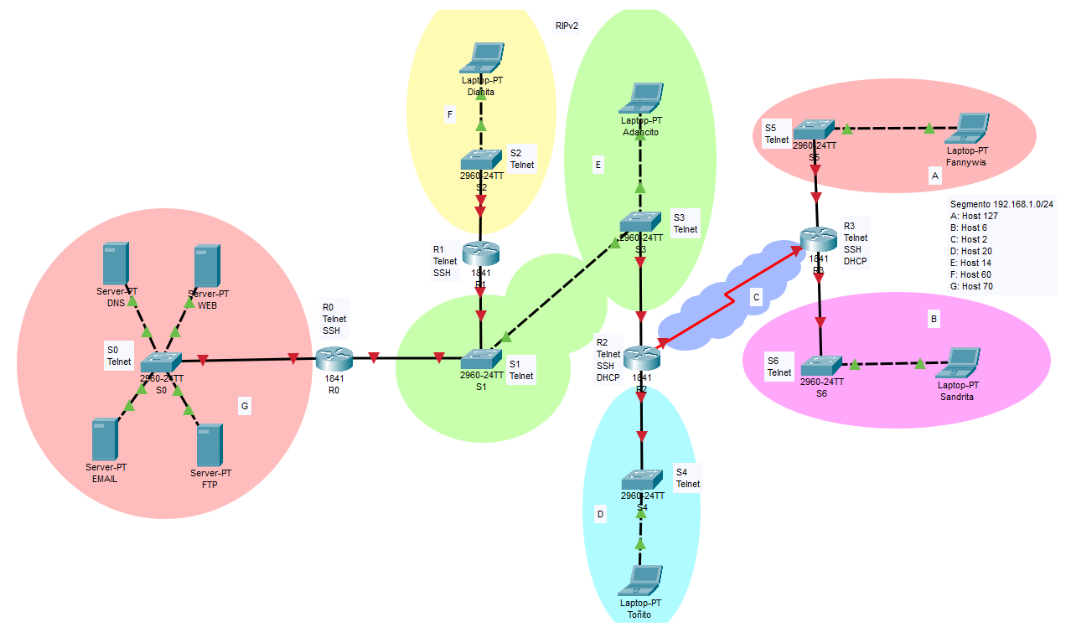
\includegraphics[width=\linewidth]{topologia}\\

\textbf{Notas}
\begin{itemize}
  \item En esta práctica todas las contraseñas de usuarios de routers, 
  switches y  \texttt{enable} son \textit{cisco}
  \item Los usuarios de routes y switches siguen la siguiente convencion
  \begin{itemize}
    \item Para el username de los router. Siempre va al inicio una \textit{u}
    seguido del hostname. De esta manera tenemos:
    \begin{itemize}
      \item \textbf{Router R0:} ur0
      \item \textbf{Router R1:} ur1
      \item \textbf{Router R2:} ur2
      \item \textbf{Router R3:} ur3
    \end{itemize}
    \item Para el username de los switches. Siempre va al inicio una \textit{u}
    seguido del hostname. De esta manera tenemos:
    \begin{itemize}
      \item \textbf{Switch S0:} us0
      \item \textbf{Switch S1:} us1
      \item \textbf{Switch S2:} us2
      \item \textbf{Switch S3:} us3
      \item \textbf{Switch S4:} us4
      \item \textbf{Switch S5:} us5
      \item \textbf{Switch S6:} us6
    \end{itemize}    
  \end{itemize}
  \item Para los correos:
  \begin{itemize}
    \item El dominio es: \texttt{feedback.com}
    \item Los usuarios y contraseñas son los mismos.
    \item Los usuarios registrados son
    \begin{itemize}
      \item dianita
      \item tonito
      \item adancito
      \item fannywis
      \item sandrita
    \end{itemize}
  \end{itemize}
\end{itemize}


\textbf{Algunas capturas de pantalla que evidencian el funcionamiento de 
algunos servicios}
\begin{enumerate}[label=\textbf{\arabic*.}]
  \item \textbf{SMTP (email)}\\[5mm]
  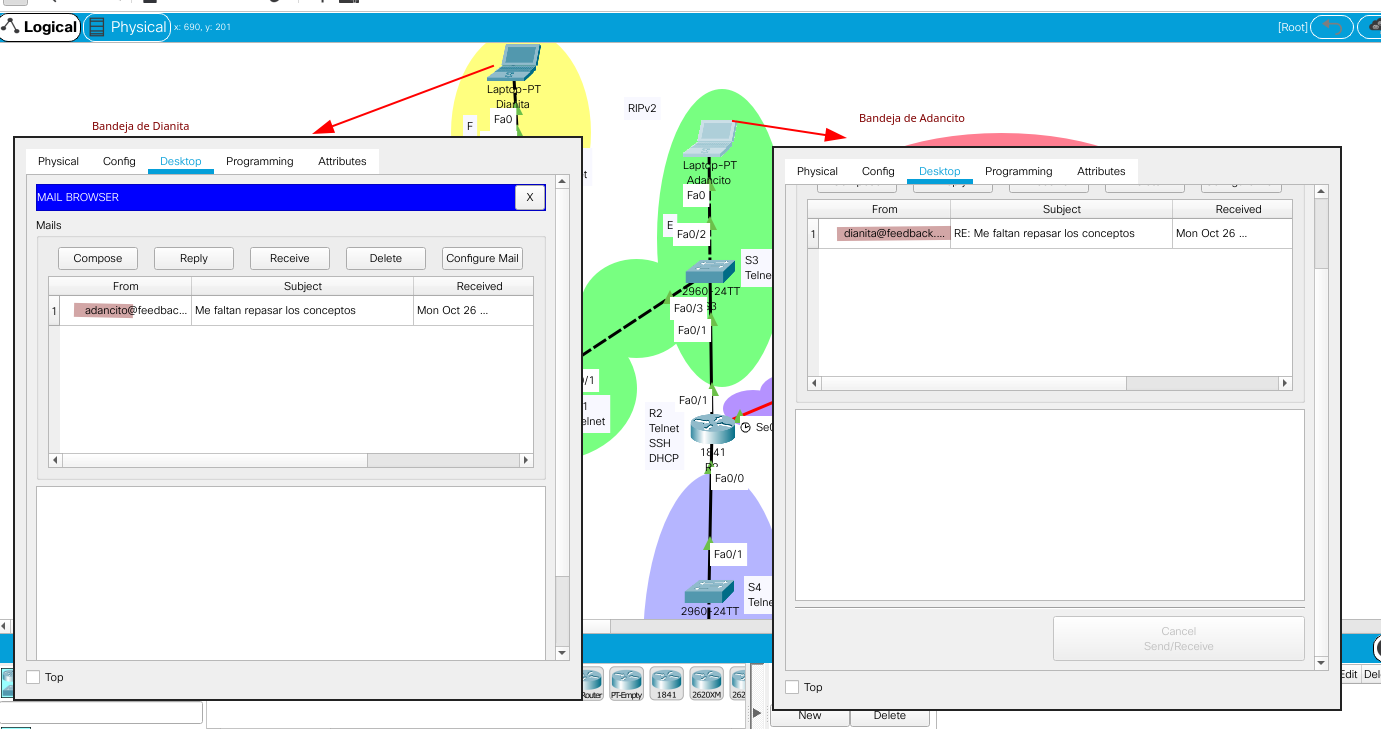
\includegraphics[width=0.9\linewidth]{correo-ev01.png}\\[5mm]
  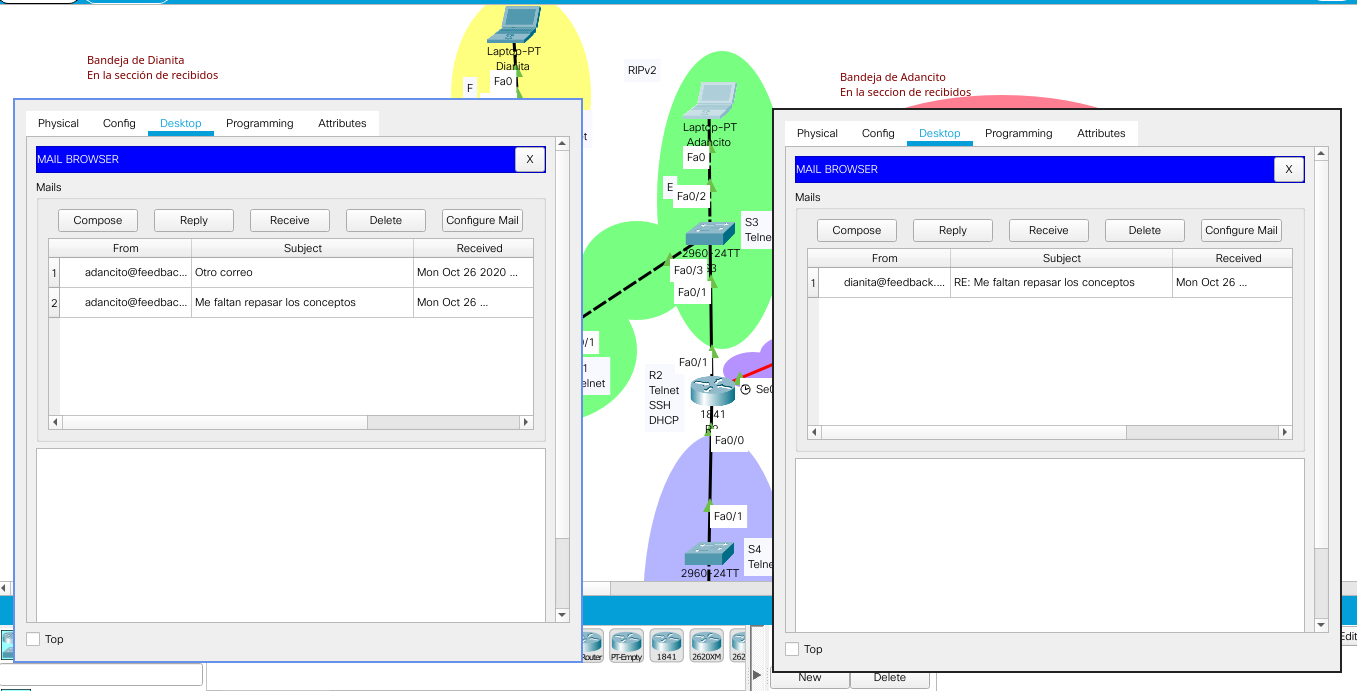
\includegraphics[width=0.9\linewidth]{correo-ev02.png}
  
  \newpage
  \item \textbf{FTP}\\[5mm]
  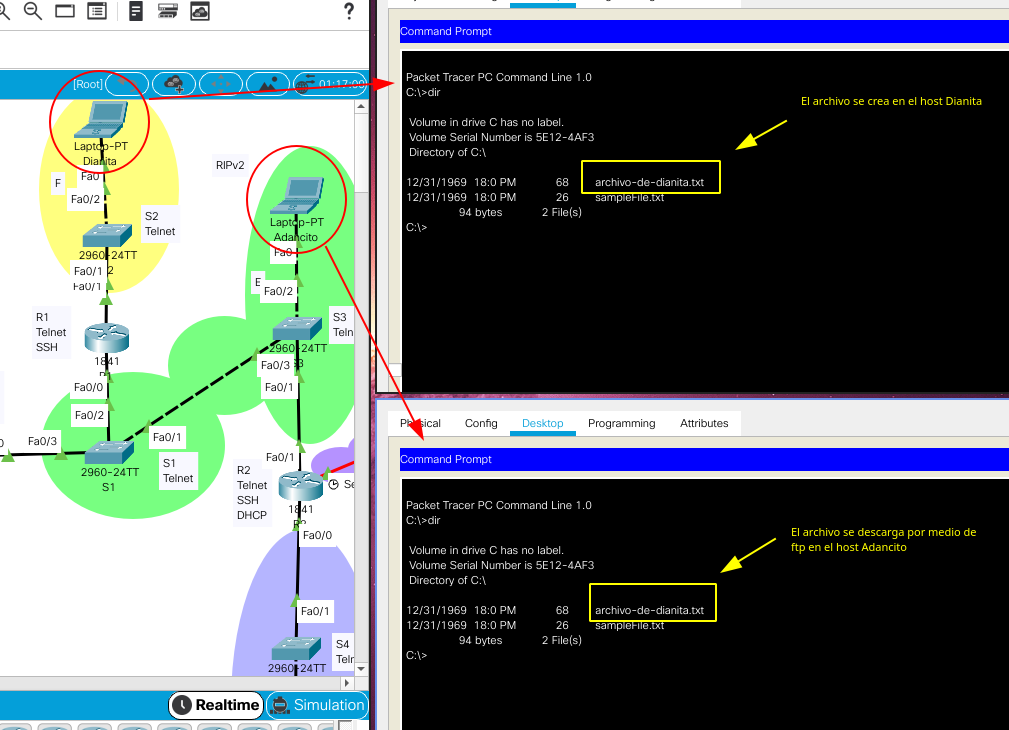
\includegraphics[width=\linewidth]{ftp-ev01.png}
  
  \item \textbf{HTTP y DNS}\\[5mm]
  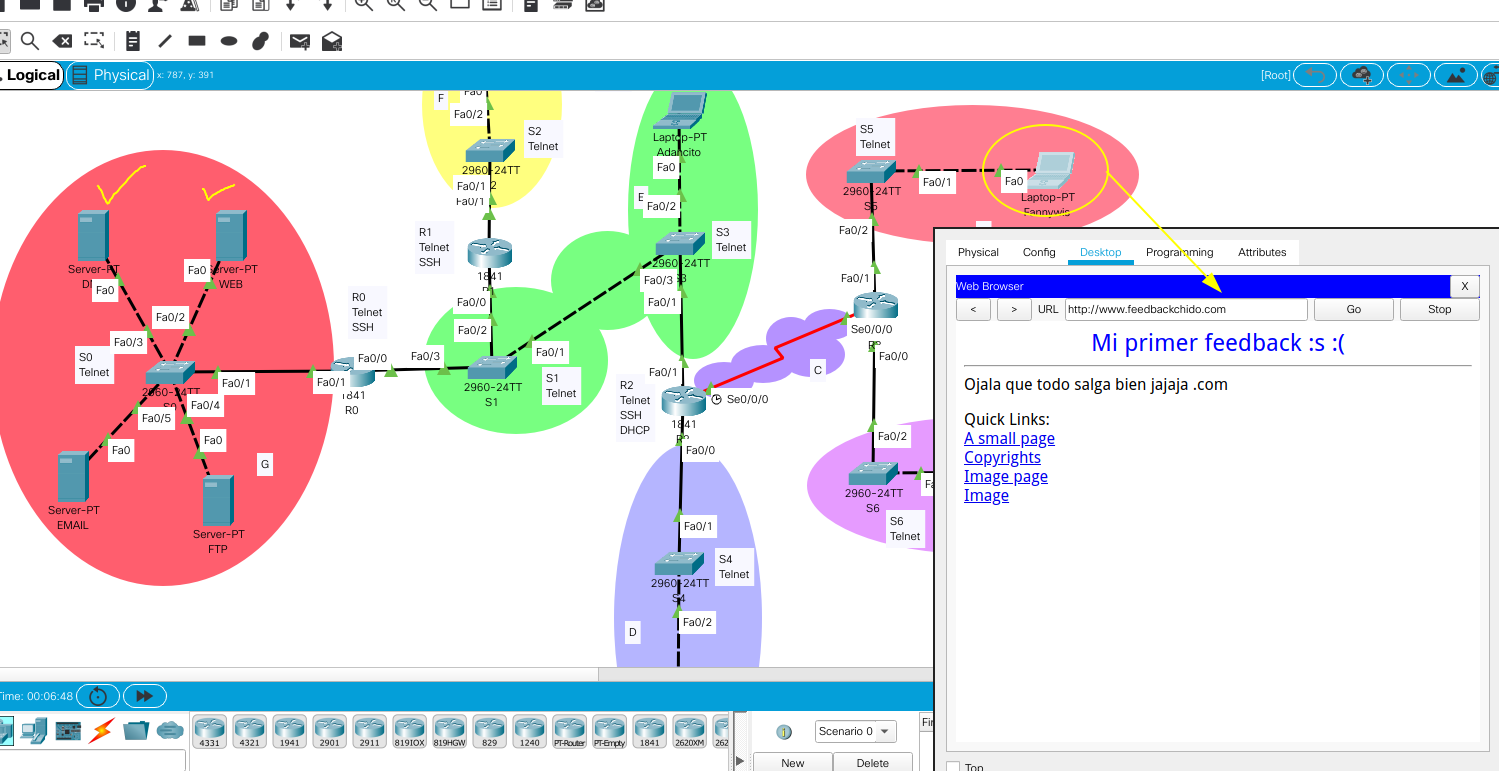
\includegraphics[width=\linewidth]{web-dns-ev01.png}
  \newpage
  \item \textbf{DHCP}\\[5mm]
  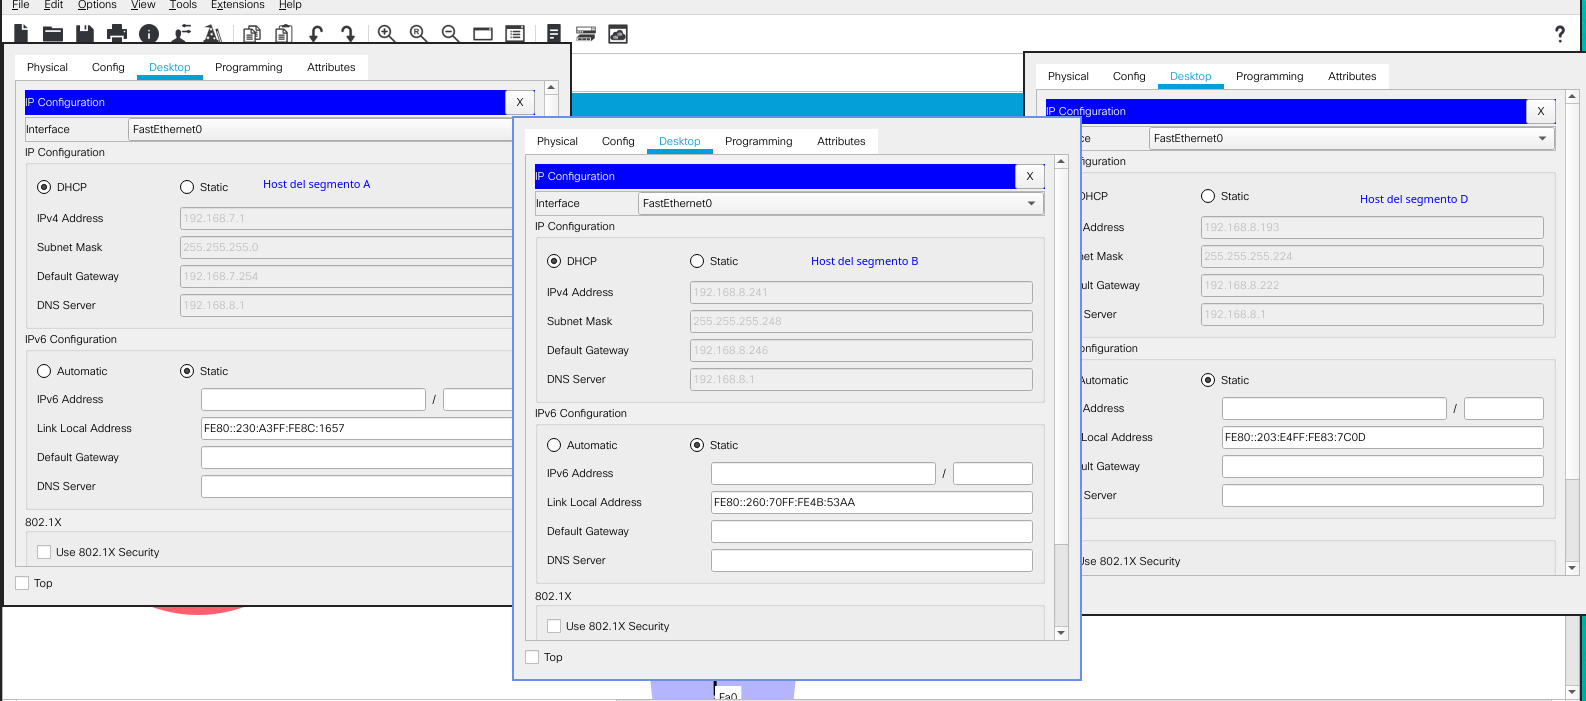
\includegraphics[width=\linewidth]{dhcp-ev01.png}
  % \newpage
  \item \textbf{Telnet de S0 a cada uno de los switches (S1,S2,S3,S4,S5,S6)}
  \\
  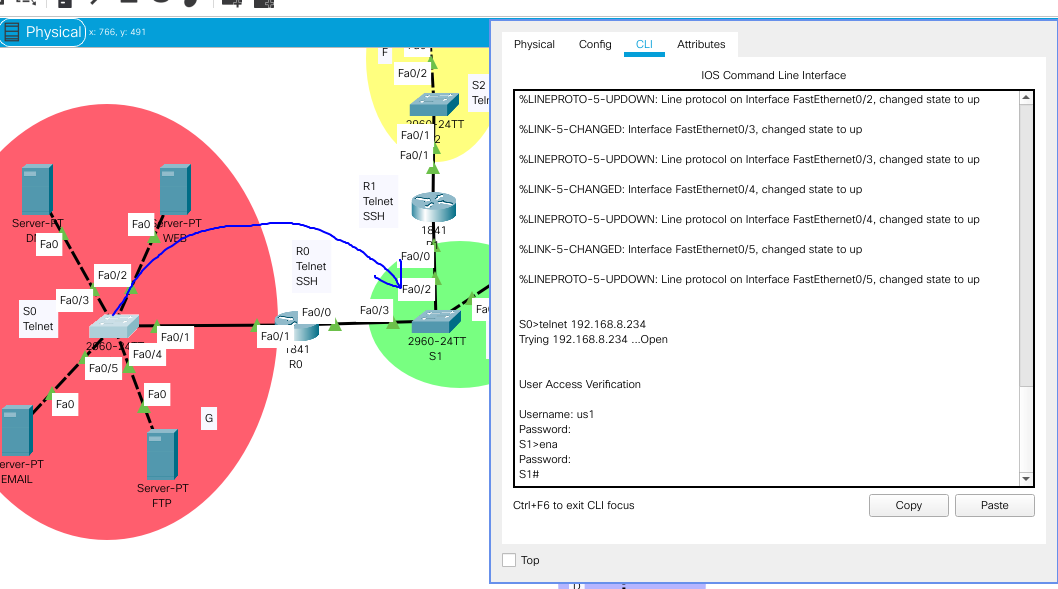
\includegraphics[width=0.8\linewidth]{telnet-s0-s1.png}\\[3mm]
  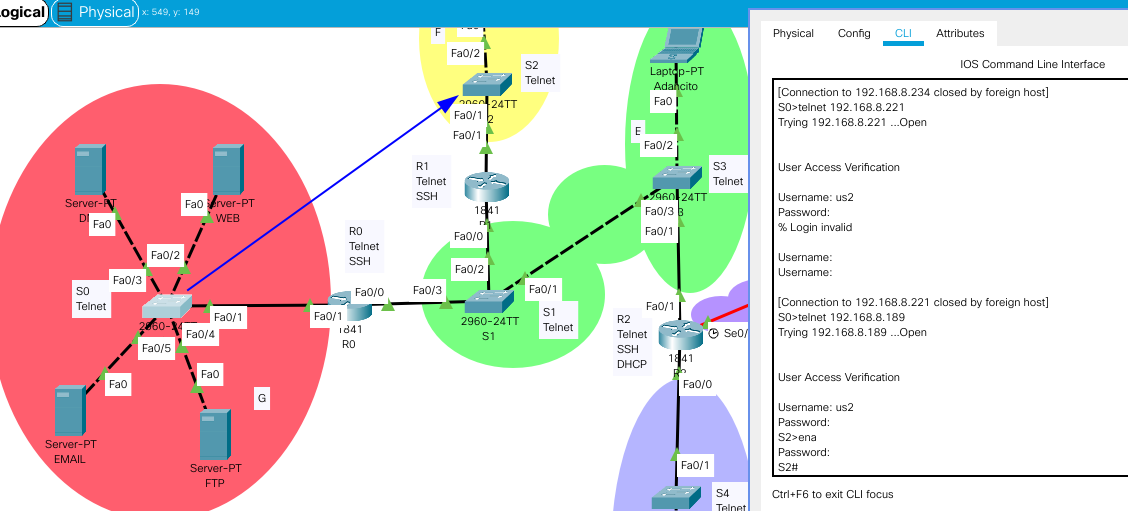
\includegraphics[width=0.8\linewidth]{telnet-s0-s2.png}\\[3mm]
  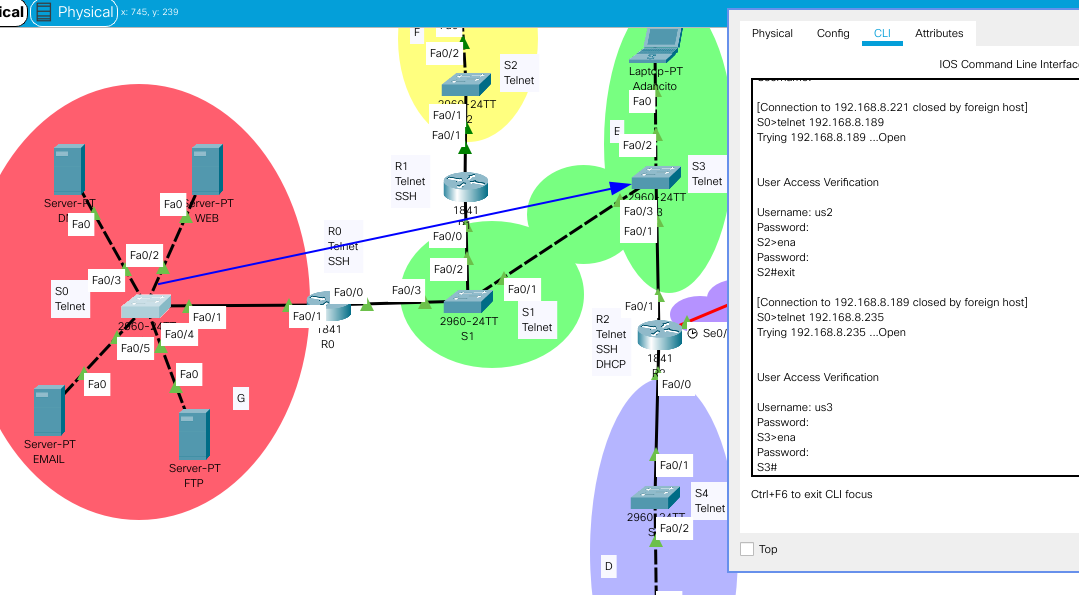
\includegraphics[width=0.8\linewidth]{telnet-s0-s3.png}\\[3mm]
  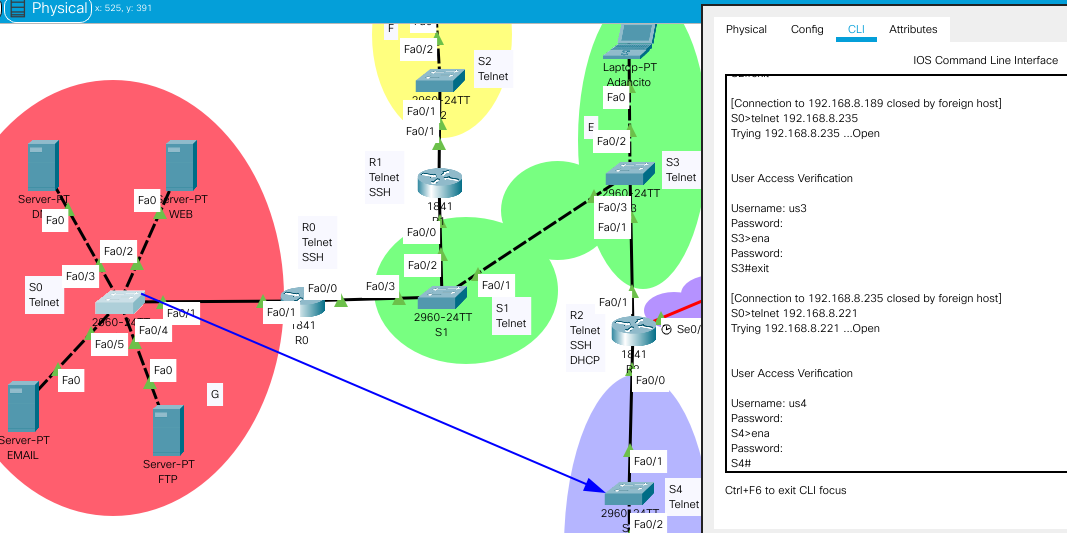
\includegraphics[width=0.8\linewidth]{telnet-s0-s4.png}\\[3mm]
  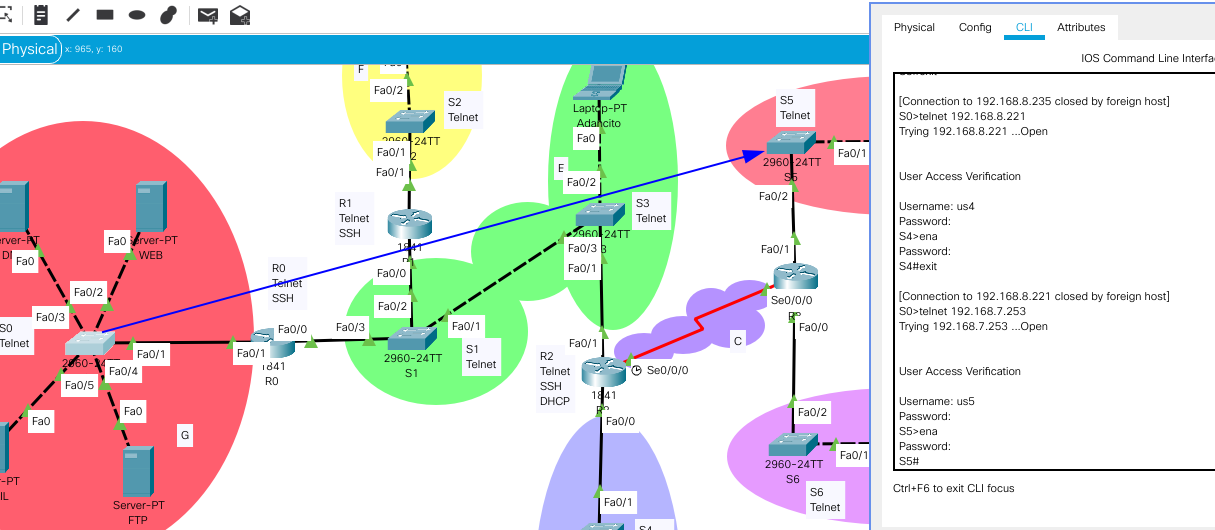
\includegraphics[width=0.8\linewidth]{telnet-s0-s5.png}\\[3mm]
  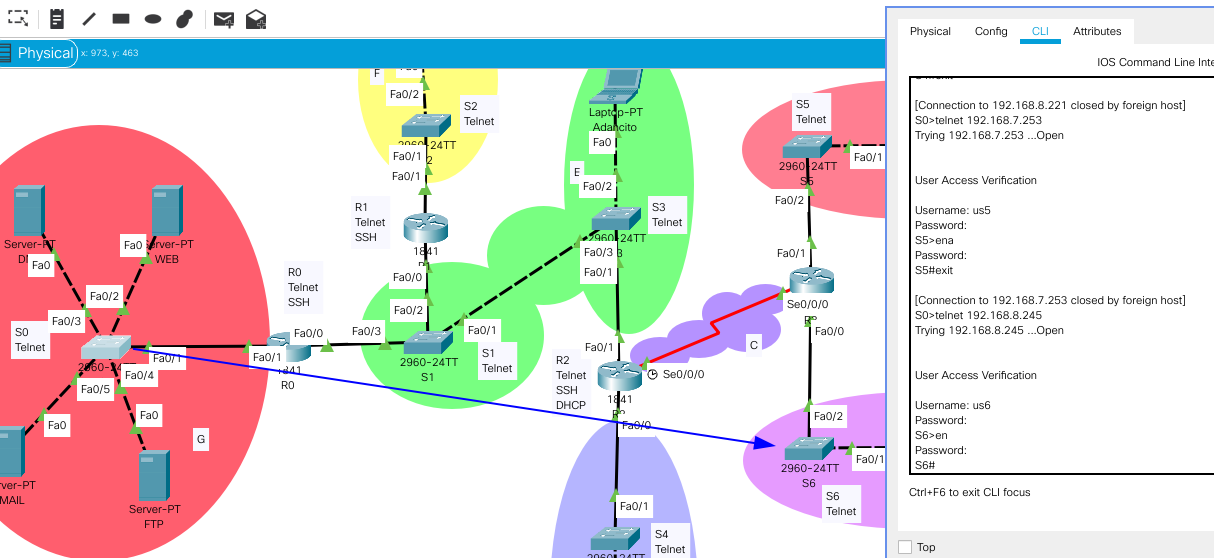
\includegraphics[width=0.8\linewidth]{telnet-s0-s6.png}\\[2cm]
  
  \item \textbf{SSH de R0 a todos los demás routers (R1,R2,R3)}\\[5mm]
  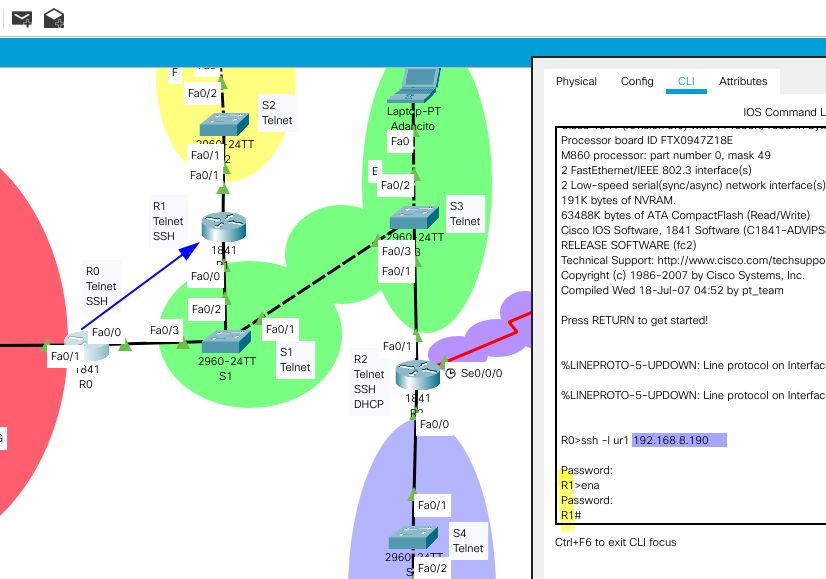
\includegraphics[width=0.8\linewidth]{ssh-r0-r1.png}\\[3mm]
  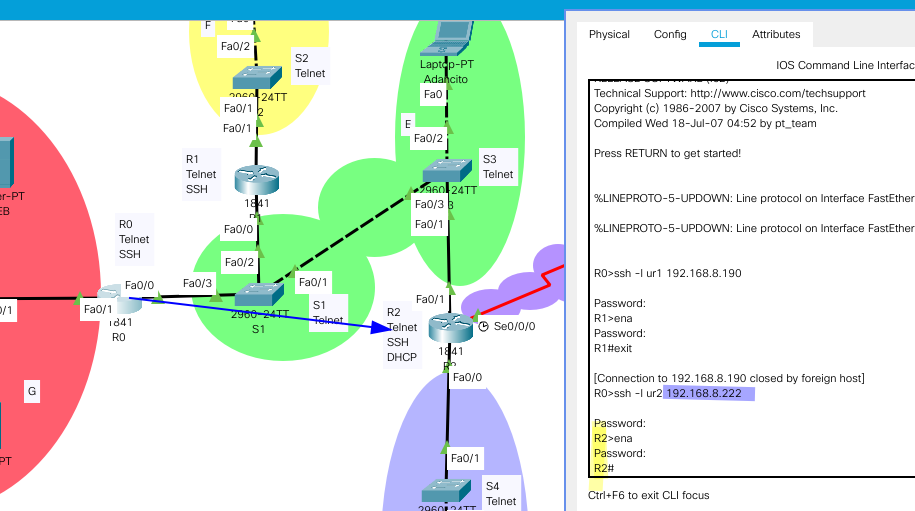
\includegraphics[width=0.8\linewidth]{ssh-r0-r2.png}\\[3mm]
  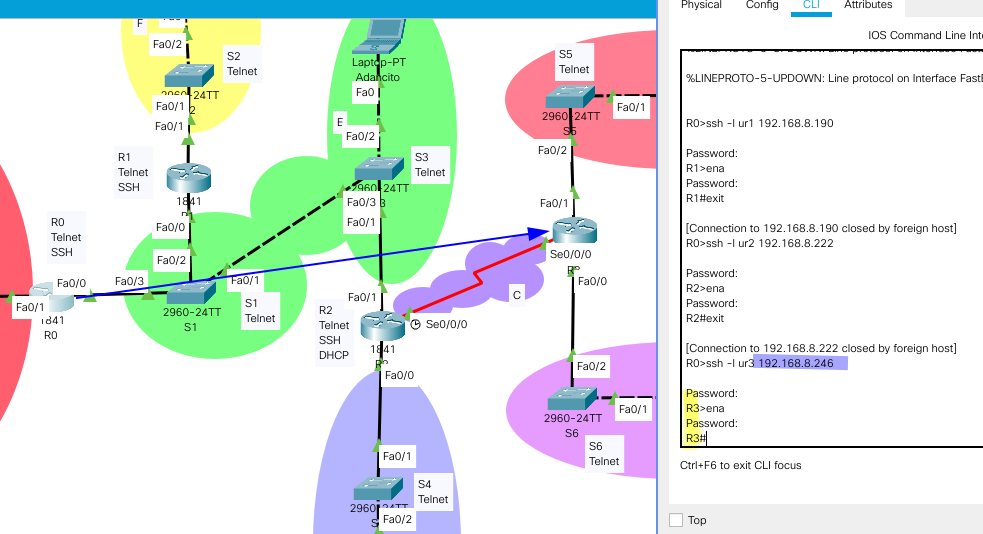
\includegraphics[width=0.8\linewidth]{ssh-r0-r3.png}\\[3mm]
  \newpage
  \item \textbf{Telnet de S1 a todos los routers}\\[5mm]
  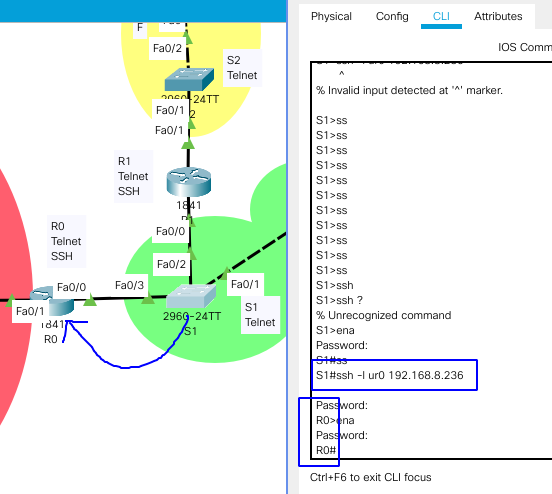
\includegraphics[width=0.8\linewidth]{ssh-s1-r0.png}\\[3mm]
  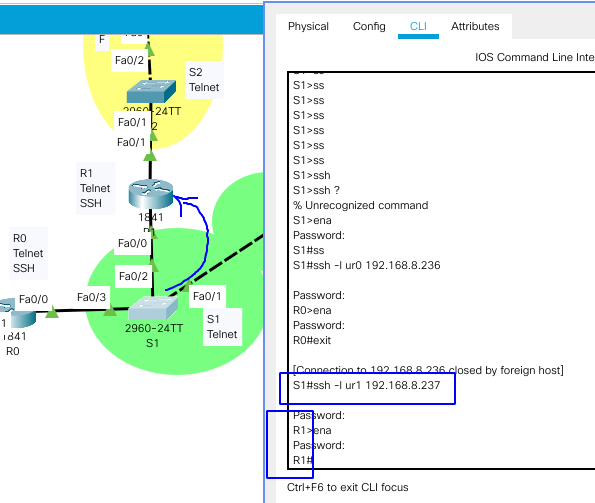
\includegraphics[width=0.8\linewidth]{ssh-s1-r1.png}\\[3mm]
  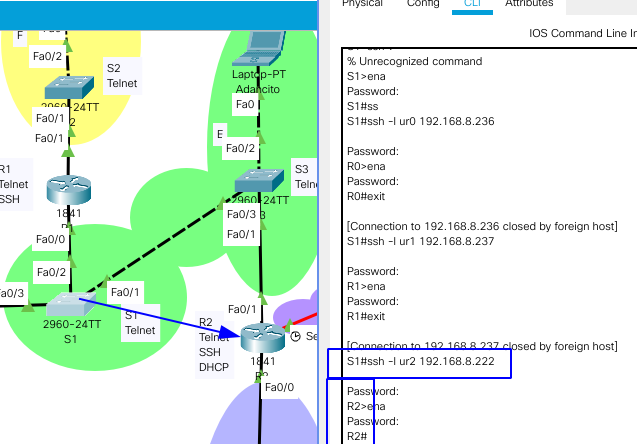
\includegraphics[width=0.8\linewidth]{ssh-s1-r2.png}\\[3mm]
  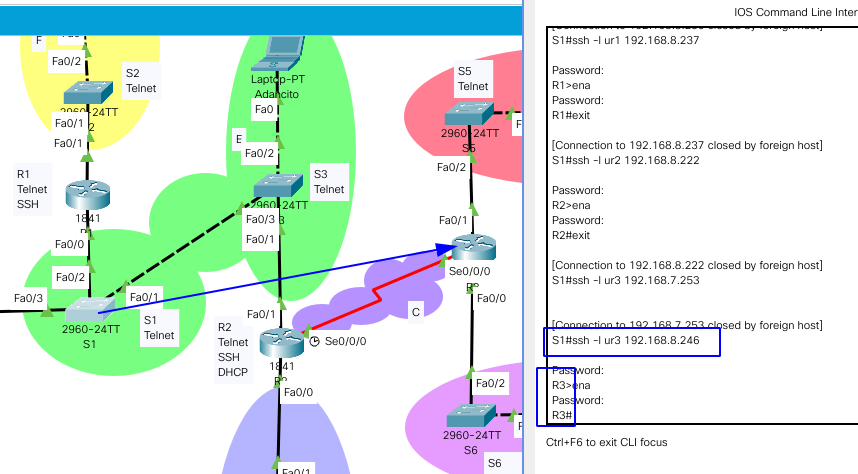
\includegraphics[width=0.8\linewidth]{ssh-s1-r3.png}\\[3mm]
\end{enumerate}

\end{document}
